\model{Array Diagrams}

Array elements are stored together in one contiguous block of memory.
To show arrays in memory diagrams, we simply draw adjacent boxes.

\begin{multicols}{2}

\begin{center}
\java{int[] nums = \{10, 3, 7, -5\};}

\vspace{1ex}
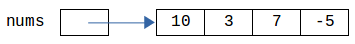
\includegraphics[scale=0.65]{array-diagram1.png}
\end{center}

\columnbreak

\begin{center}
\java{double[] stats = new double[3];}

\vspace{1ex}
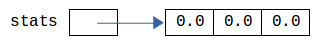
\includegraphics[scale=0.65]{array-diagram2.png}
\end{center}

\end{multicols}


\quest{15 min}


\Q What is the default value for array elements?

\begin{answer}[3em]
Zero or equivalent value, depending on the data type.
For numeric types like {\tt int} and {\tt double}, the default is 0; for {\tt boolean}, it's {\tt false}; for {\tt char}, it's {\tt \qs{\bs u0000}\qs}; for reference types, it's {\tt null}.
\end{answer}


\Q Draw a memory diagram for the following arrays.
(\textit{Hint:} You should have no empty boxes.)

\begin{minipage}{0.46\linewidth}

\begin{enumerate}

\item
\begin{javalst}
int[] sizes = new int[5];
sizes[2] = 7;
\end{javalst}

\item
\begin{javalst}
double[] costs = new double[4];
costs[0] = 0.99;
\end{javalst}

\item
\begin{javalst}
String[] names = {"Anita"};
\end{javalst}

\end{enumerate}

\end{minipage}
\hfill
\begin{minipage}{0.53\linewidth}
\note{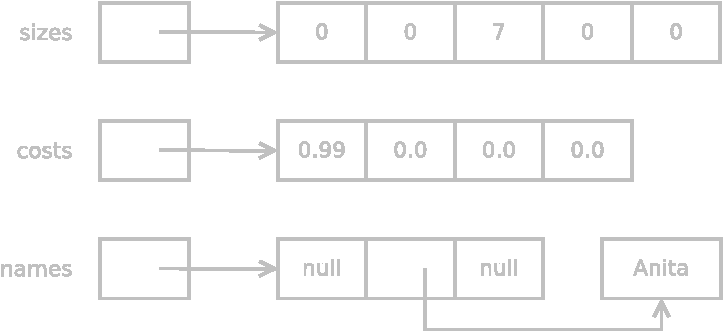
\includegraphics[width=\linewidth]{decl-array.pdf}}
\end{minipage}


\Q Like strings, arrays are reference types. What is the value of an array {\it variable}?

\begin{answer}[3em]
An integer representing the memory location of the array.
\end{answer}


\Q Does the statement \java{int[] copy = nums;} create a new array? Justify your answer.

\begin{answer}[3em]
No. If you assign one array variable to another, you're only copying the reference, not the array itself.
\end{answer}


\Q Draw a memory diagram of the following array.
(\textit{Hint:} You should have four arrows.)

\begin{javalst}
String[] greek = {"alpha", "beta", "gamma"};
\end{javalst}

\vspace{1em}
\hspace{2em}
\note{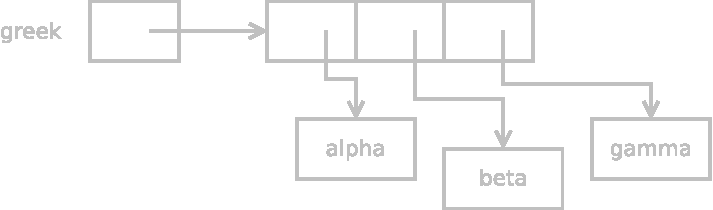
\includegraphics[height=6em]{string-array.pdf}}
